\begin{spacing}{1}
    \chapter*{Abstract}
\end{spacing}
\begin{wrapfigure}{r}{0.3\textwidth}
    \begin{center}
      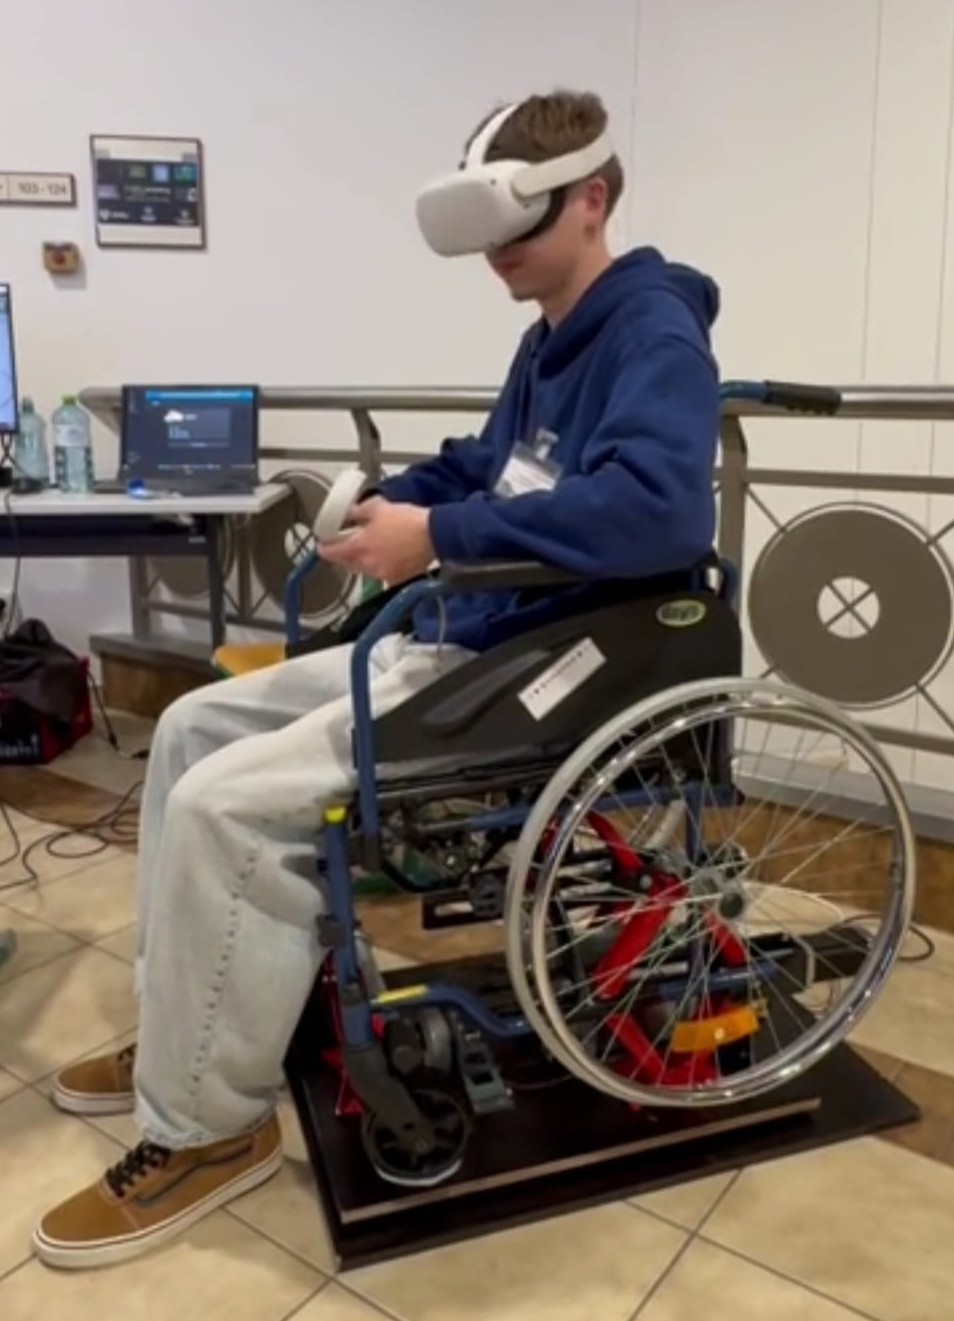
\includegraphics[width=0.4\textwidth]{pics/tdot.jpg}
    \end{center}
\end{wrapfigure}
This thesis investigates how immersive virtual reality (VR) applications can be used to make barriers to wheelchair mobility in urban environments tangible and to raise awareness of the challenges faced by wheelchair users. On the one hand, the focus is on designing a realistic 3D world and facilitating interaction within the virtual environment. On the other hand, a hardware simulator is developed to replicate wheelchair movements.

To this end, a VR environment was created that depicts typical everyday situations, such as navigating streets or overcoming curbs that are too high. In addition, a movable simulator was designed that, in combination with a real wheelchair, provides physical feedback such as tilting and vibrations. This enhances the virtual experience with haptic sensations, making it more realistic.

The results show that the combination of virtual and physical simulation can create a particularly immersive user experience that goes beyond conventional VR applications. Furthermore, the developed solution helps to foster understanding of existing barriers and can be used as a tool for awareness-raising, training, and planning accessible infrastructure.

\newpage
\begin{spacing}{1}
    \chapter*{Zusammenfassung}
\end{spacing}
\begin{wrapfigure}{r}{0.3\textwidth}
    \begin{center}
      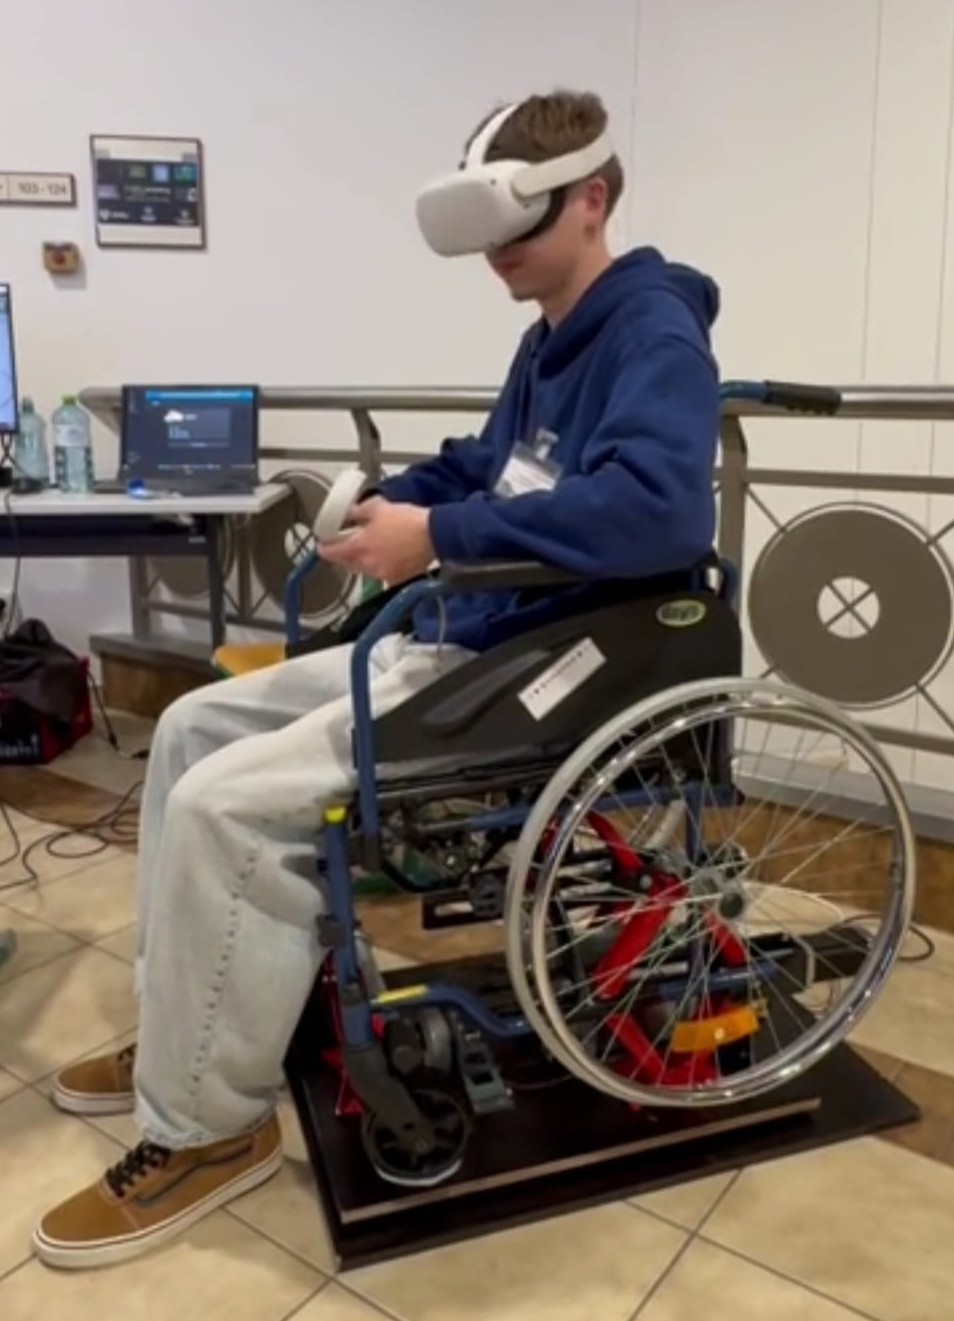
\includegraphics[width=0.4\textwidth]{pics/tdot.jpg}
    \end{center}
\end{wrapfigure}
Die vorliegende Arbeit untersucht, wie immersive Virtual-Reality-Anwendungen genutzt werden können, um Barrieren für die Fortbewegung im Rollstuhl im urbanen Umfeld erfahrbar zu machen und ein Bewusstsein für die Herausforderungen von Rollstuhlfahrenden zu schaffen. Zum einen liegt der Fokus auf der Gestaltung einer realistischen 3D-Welt sowie der Interaktion in der virtuellen Realität. Zum anderen wird ein Hardware-Simulator entwickelt, der Bewegungen im Rollstuhl simuliert.

Hierzu wurde eine VR-Umgebung geschaffen, die typische Alltagssituationen wie das Navigieren durch Straßen oder das Überwinden von zu hohen Bordsteinen abbildet. Ergänzend dazu wurde ein beweglicher Simulator konzipiert, die in Kombination mit einem realen Rollstuhl physische Rückmeldungen wie Neigungen und Vibrationen erzeugt. Dadurch wird die virtuelle Erfahrung durch haptische Eindrücke erweitert und realistischer gestaltet.

Die Ergebnisse zeigen, dass durch die Verbindung von virtueller und physischer Simulation ein besonders intensives Nutzererlebnis erzeugt werden kann, das über klassische VR-Anwendungen hinausgeht. Zudem trägt die entwickelte Lösung dazu bei, das Verständnis für bestehende Barrieren zu fördern und kann als Werkzeug für Sensibilisierung, Ausbildung und die Planung barrierefreier Infrastrukturen eingesetzt werden.
